The MIDI converter layers consists of single component i.e. MIDI encoder. The encoder takes the signals passed on by the receptors and changes it into MIDI signals. Those MIDI signals are forwarded towards MIDI decoder of sound module.

\subsection{MIDI encoder}
The MIDI encoder gets the signal from the laser receptors, converts it to MIDI data and sends to the Raspberry Pi for the output. This converts the laser receptor signals to MIDI data in order to convert it to sound data.  

\begin{figure}[h!]
	\centering
 	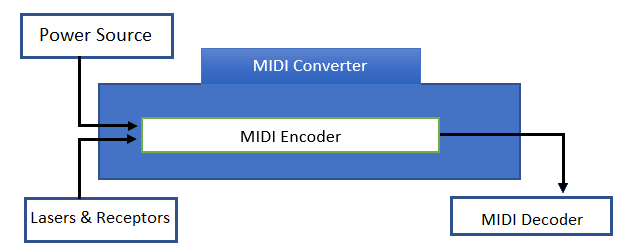
\includegraphics[width=0.60\textwidth]{images/MIDI_encoder}
 \caption{MIDI encoder subsystem diagram}
\end{figure}

\subsubsection{Assumptions}
The MIDI encoder is connected to the Pi and the laser receptors via cable. It also has a built-in software that converts the data automatically.

\subsubsection{Responsibilities}
The laser receptors, when it detects an interference, sends signal to the MIDI encoder. Here, the encoder converts the signal data it received to a MIDI data so it can be manipulated to different sounds with the sound modules.

\subsubsection{Subsystem Interfaces}
It receives the laser signals and converts it into MIDI signals which it sends to the pi.

\begin {table}[H]
\caption {Subsystem interfaces} 
\begin{center}
    \begin{tabular}{ | p{1cm} | p{6cm} | p{3cm} | p{3cm} |}
    \hline
    ID & Description & Inputs & Outputs \\ \hline
    \#01 & MIDI Encoder & \pbox{3cm}{ Laser Signals} & \pbox{3cm}{MIDI signals}  \\ \hline
    \end{tabular}
\end{center}
\end{table}


